
En este capítulo introducimos conceptos acerca del aprendizaje automático, la rama de la inteligencia artificial que se ocupa de inferir conocimiento sin necesidad de una programación explícita. Además, se estudia el problema de clasificación y cómo es afectado por la dimensionalidad de los datos. Llegamos así a presentar el problema principal que trata este trabajo: la reducción de la dimensionalidad. Por último, se expone un algoritmo clásico de optimización, gradiente descendente, que servirá como base para los utilizados en Deep Learning.

\section{Introducción}\label{introducciuxf3n}


%\textcolor{red}{qué aborda este capítulo y qué estructura: visión general}

%El aprendizaje profundo o Deep Learning comprende una clase de técnicas
%englobadas dentro del aprendizaje automático. Esta sección introduce los
%conceptos básicos de aprendizaje automático, que son comunes a todas las
%técnicas desarrolladas en el ámbito.

Un \emph{algoritmo de aprendizaje} es, según \textcite{mitchell1997}, un
programa cuyo rendimiento respecto de un conjunto de tareas \(T\) y una
medida de rendimiento \(P\) mejora tras conocer una experiencia \(E\).
En ese caso, se dice que el algoritmo ha \emph{aprendido} de dicha
experiencia.

Estas tareas y experiencias pueden ser de muy diversas clases, lo que
propicia la aparición de algoritmos y técnicas de aprendizaje diferentes
que tratan de abordarlas. Estos algoritmos computacionales son
necesarios cuando la complejidad o el tamaño de la tarea impide tratarla
con técnicas manuales.

Entre las tareas de aprendizaje que se presentan en la literatura se
incluyen:

\begin{itemize}
\tightlist
\item
  clasificación
\item
  regresión
\item
  detección de anomalías
\item
  agrupamiento (\emph{clustering})
\item
  reducción de dimensionalidad
\item
  detección y eliminación de ruido
%\item traducción automática
\end{itemize}


\section{Tipos de aprendizaje}\label{sec:learning-types}

La mayoría de \emph{experiencias} de las que puede
aprender un algoritmo permite categorizar el aprendizaje en dos grandes clases:
supervisado y no supervisado.

% \textcolor{red}{reestructurar}

\subsection{Aprendizaje supervisado}

En aprendizaje supervisado, se le proporciona al algoritmo un conjunto
de ejemplos para los cuales la tarea está resuelta. Así, se pretende que
aprenda a realizar la misma tarea para nuevas muestras.

Algunos problemas concretos en los que se realiza esta clase de aprendizaje son:
\begin{itemize}
\item Clasificación: el programa debe deducir una etiqueta o clase para cada instancia, y para ello el aprendizaje se suele realizar mediante un conjunto de ejemplos que ya tienen asignada su etiqueta. En la \autoref{sec:clasif} se desarrolla este problema en mayor detalle.
\item Regresión: consiste en asignar un valor real a cada nuevo conjunto de valores de entrada, habiendo aprendido de muestras que ya tenían un valor asociado.
\item Predicción de series temporales: se trata de predecir el valor de una variable en el futuro, conociendo su valor en distintos puntos del pasado.
\end{itemize}

\subsection{Aprendizaje no supervisado}\label{aprendizaje-no-supervisado}

La modalidad no supervisada involucra a tareas de las que el algoritmo
no tiene ejemplos resueltos. La experiencia que se le
proporciona puede estar basada en otras características de los datos.

Algunas de las tareas donde se utiliza aprendizaje no supervisado son:
\begin{itemize}
\item Agrupamiento o
\emph{clustering}: se proporcionan al algoritmo datos sin
clasificar que debe subdividir en diferentes conjuntos de forma que los
datos del mismo conjunto sean más similares entre sí que entre elementos
de distintos conjuntos.
\item Reglas de asociación: el programa debe extraer relaciones relevantes entre los
  atributos del conjunto de datos que aporten información útil y novedosa acerca de la
  situación estudiada.
\item Aprendizaje de características: se aportan datos sin etiquetar, para los que el algoritmo debe extraer características representativas. También se da este problema en el aprendizaje supervisado, cuando los datos están etiquetados.
\end{itemize}

El aprendizaje no supervisado abarca multitud de problemas ampliamente
estudiados que tienen diversas aplicaciones presentes en distintos
campos, como el tratamiento de imágenes y reconocimiento de objetos
\autocite{ranzato}, análisis semántico \autocite{hofmann} y sintáctico
del lenguaje \autocite{brent} o el preprocesamiento de datos y
pre-entrenamiento para una posterior fase de aprendizaje
\autocite{erhan2009}.

\section{Problema de clasificación}\label{sec:clasif}

Un problema clásico en el aprendizaje automático es el de clasificación. Se trata de una tarea de aprendizaje supervisado que consiste en aprender acerca de la etiqueta o clase de una secuencia de muestras clasificadas, para después ser capaz de predecir el valor de dicha etiqueta en nuevas instancias sin clasificar.

La clasificación tiene multitud de aplicaciones en diversos ámbitos.
Algunos ejemplos son el diagnóstico de enfermedades \autocite{kononenko2001}, la
detección de fraude \autocite{phua2010} y la clasificación de mensajes de correo \autocite{cohen1996}.

\subsection{Definición}

Una formulación sencilla del problema es la siguiente:

\defineb
Sean \(A_1, A_2, \dots A_f\) conjuntos no vacíos llamados
\emph{atributos de entrada}. Llamaremos \emph{espacio de atributos} (o
\emph{espacio de características}) a
\(\mathcal A=A_1\times A_2\times\dots\times A_f\).

Sea $L$ un conjunto finito al que denominaremos \emph{conjunto de etiquetas}.

Sea \(D\subset \mathcal A\times L\) un subconjunto finito del espacio de
atributos, lo llamaremos \emph{conjunto de instancias} o \emph{dataset}.

Decimos que la tripleta \(\mathcal P=\left(\mathcal A, L, D\right)\) es
un \emph{problema de clasificación}. \definee

\defineb
Dado un problema de clasificación \(\left(\mathcal A, L, D\right)\), un
\emph{clasificador} es una aplicación \(c:\mathcal A\rightarrow L\).
\definee

Así, el objetivo que se persigue al abordar un problema de clasificación
\(\mathcal P\) es encontrar el clasificador \(c\) que mejor se adapte al
problema, según una o varias métricas de evaluación. Intuitivamente, el
procedimiento por el que se obtenga dicho clasificador debe ser capaz de
utilizar la información de las instancias en el dataset \(D\) para
predecir una clase en nuevas instancias del espacio de atributos.

Atendiendo a la estructura de $L$, es decir, el número de características que estarán ausentes en los nuevos datos y sus posibles valores, distinguiremos los siguientes tipos de clasificación:
\begin{itemize}
\item Binaria: implica clasificar en 2 clases (generalmente significan que una condición es verdadera o falsa), utilizando una característica que tome únicamente dos valores. Así, $L = \{0,1\}$.
\item Multiclase: en este caso habrá más de dos clases, pero cada instancia pertenecerá a una y solo una de ellas, por lo que se usará una característica que contenga tantos valores como clases: $L=\{0, 1,\dots, l\}$.
\item Multietiqueta: en esta situación, cada instancia puede asociarse a más de una etiqueta, por tanto se usarán tantos atributos como etiquetas, cada uno de ellos conteniendo dos valores: $L=\{0,1\}\times\dots\times\{0,1\}$.
\item Multidimensional: se trata de una generalización del caso multietiqueta donde cada una de las etiquetas toma valores en un conjunto finito arbitrario, esto es, $L=\{0,\dots, \lambda_1\}\times\dots\times\{0,\dots, \lambda_l\}$.
\end{itemize}


Las definiciones previas componen una formalización simple del problema
de clasificación. Una modelización más detallada y con consecuencias
teóricas de interés se encuentra en la teoría de aprendizaje PAC
\autocite{shwartz2014}. De esta teoría además se extraen algunos resultados
relevantes. Por un lado, el hecho de que los algoritmos sean capaces de generalizar
un modelo adecuado a partir de una cantidad finita de muestras. Por contraposición,
considerados sobre el conjunto de todas las distribuciones de datos
posibles, todos los algoritmos de clasificación presentan en media la
misma tasa de error en la predicción de clases para nuevos ejemplos
(hecho conocido como el teorema de \textit{No Free Lunch}\textcolor{red}{ref!}).

%\begin{example}
%\textcolor{red}{Si se me ocurre un ejemplo, añadirlo.}
%\end{example}

\subsection{Estructura del espacio de
atributos}\label{estructura-del-espacio-de-atributos}

En principio no tenemos por qué asumir una estructura algebraica para el
espacio de atributos \(\mathcal A\), pero la mayoría de algoritmos
necesitarán una forma de medir similitud entre instancias. Para ello,
normalmente se puede utilizar una distancia \(d\), de forma que
\((\mathcal A,d)\) sea un espacio métrico. Para el uso de un conjunto de
datos en redes neuronales, sin embargo, convendrá suponer además
\(\mathcal A\subset \mathbb R^f\).

\section{Problema de reducción de
dimensionalidad}\label{sec:red-dim}

Es común encontrar problemas de clasificación donde el espacio de
atributos posee una alta dimensionalidad. Por ejemplo: conjuntos de
datos extraídos de texto, donde cada atributo representa la aparición de
una palabra en un documento; conjuntos basados en imágenes donde cada
atributo representa un píxel \autocite{mnist}, o datos que
expresan características genéticas \autocite{clarke2008}.

Como consecuencia del \autoref{th:dim-curse}, al aumentar la dimensionalidad de los conjuntos de datos se pierde significatividad en las distancias, en el sentido de que, para una instancia de la muestra dada, la instancia más cercana y la instancia más lejana están a distancias muy similares.

Las distancias entre puntos en el espacio de atributos son utilizadas en
multitud de algoritmos de aprendizaje automático, entre los cuales el
ejemplo más claro es la técnica del Vecino más cercano
\autocite{peterson2009}, aplicada en clasificación en el algoritmo de los k-vecinos más cercanos.

Ante un conjunto de datos de alta
dimensionalidad, podemos discernir dos vías de acción:
\begin{itemize}
\tightlist
\item
  Estudiar y transformar los datos manteniendo la dimensionalidad, para
  que las distancias entre puntos sean significativas.
\item
  Reducir la dimensionalidad de los datos, manteniendo toda la
  información útil que sea posible.
\end{itemize}
En nuestro caso, utilizaremos algunas técnicas de Deep Learning para
operar de la segunda forma, comprimiendo los datos en un espacio de
menor dimensionalidad.

Con el objetivo de reducir la dimensionalidad de un conjunto de datos,
se alteran las características del mismo en un proceso denominado
\emph{extracción de características}, que comprende dos procesos alternativos que en ocasiones se combinan
\autocite{guyon2006}:

\begin{enumerate}
\def\labelenumi{\arabic{enumi}.}
\tightlist
\item
  \textbf{Construcción de características}. Se transforman los datos,
  operando entre las características para hallar un nuevo conjunto de
  atributos que posiblemente facilite el aprendizaje de los datos.
\item
  \textbf{Selección de características}. Se escogen las características
  que se consideren más relevantes para obtener información, y se
  descartan las que no son útiles.
\end{enumerate}

En ocasiones únicamente es necesaria una selección de características y
se puede obviar la primera fase. En otras, la propia construcción de
características sirve para sustituir a las originales y por tanto
incluye la segunda etapa.

La selección de características se puede realizar mediante muy distintas
técnicas, desde metaheurísticas hasta basadas en teoría de la
información \autocite{molina2002}.

Por otro lado, la construcción de características se pone en práctica de
formas de variable complejidad. De entre las más sencillas cabe
mencionar la normalización, la discretización, o tomar combinaciones
lineales de las características existentes. Además, se pueden destacar
técnicas más avanzadas como Isomap \autocite{tenenbaum2000}, Locally
Linear Embedding \autocite{roweis2000}, o los autoencoders
\autocite{hinton2006autoencoder}. Este trabajo se centrará en estudiar
estos últimos.

\section{Métodos de optimización: gradiente
descendente}

\label{sec:grad-desc}

Gran parte del trabajo computacional en aprendizaje automático requiere
optimizar funciones, es decir, encontrar el máximo o el mínimo de una
función \(f:\RR^n\rightarrow \RR\). Dicha función se suele denominar
\emph{función objetivo}, y normalmente corresponde al coste o error de
aprendizaje de un algoritmo. En lo sucesivo, se supondrá que el objetivo
a conseguir es encontrar el mínimo de la función \(f\). Los resultados y
algoritmos son análogos para la búsqueda de un máximo, simplemente
cambiando el signo de \(f\).

Estudiemos una simplificación del problema de optimización a una
variable. Sea \(f:[a,b]\rightarrow\RR\) continua en \([a,b]\) y
derivable con derivada continua en \(]a,b[\). Por un resultado elemental
de análisis matemático, es conocido que un extremo (máximo o mínimo)
local en una función derivable se encuentra siempre en un punto de
derivada cero. Además, por el teorema del valor medio, para
\(\varepsilon>0\) se tiene que
\[\exists c\in ]a, a+\varepsilon[ :\ f(a+\varepsilon)-f(a)=\varepsilon f'(c)\Rightarrow f(a+\varepsilon)=f(a) + \varepsilon f'(c)\]
y, por continuidad de \(f'\), si \(\varepsilon\) es suficientemente
pequeño el signo de la derivada no cambiará entre \(a\) y \(c\). Así,
\[f'(a)<0\Rightarrow f(a+\varepsilon) < f(a);\ f'(a)>0\Rightarrow f(a+\varepsilon) > f(a).\]

El método del gradiente descendente, en una variable, consiste en
evaluar \(f\) a pequeños saltos de \(\varepsilon\) y consultar la
derivada para decidir el sentido del próximo salto.

En el caso de varias variables, el algoritmo es muy similar. Sabiendo
que el gradiente de una función real de varias variables
\(f:\RR^n\rightarrow \RR\) es un vector que apunta en la dirección y
sentido de la mayor pendiente (derivada direccional) ascendente de la
función, el gradiente cambiado de signo estará posicionado en el sentido
de mayor pendiente descendente.

Así, suponiendo la suficiente regularidad para \(f\) y que se puede
evaluar tanto la función como su derivada en cualquier punto del
dominio, se puede aplicar el algoritmo de gradiente descendente,
originalmente debido a \textcite{cauchy1847}.

El algoritmo generalizado consiste en, a cada paso determinado por un
punto \(x\) del dominio, consultar el gradiente de \(f\) en \(x\),
\(\nabla f(x)\), y ``saltar'' una cantidad \(\varepsilon>0\) en su
dirección y en el sentido contrario: \[x' = x - \varepsilon\nabla f(x)\]
Al escalar \(\varepsilon\) se le suele llamar \emph{tasa de
aprendizaje}.

El algoritmo termina cuando \(\nabla f(x)\) es el vector cero o muy
cercano a cero, con una tolerancia dada.

\begin{figure}[hbtp]
  \centering
  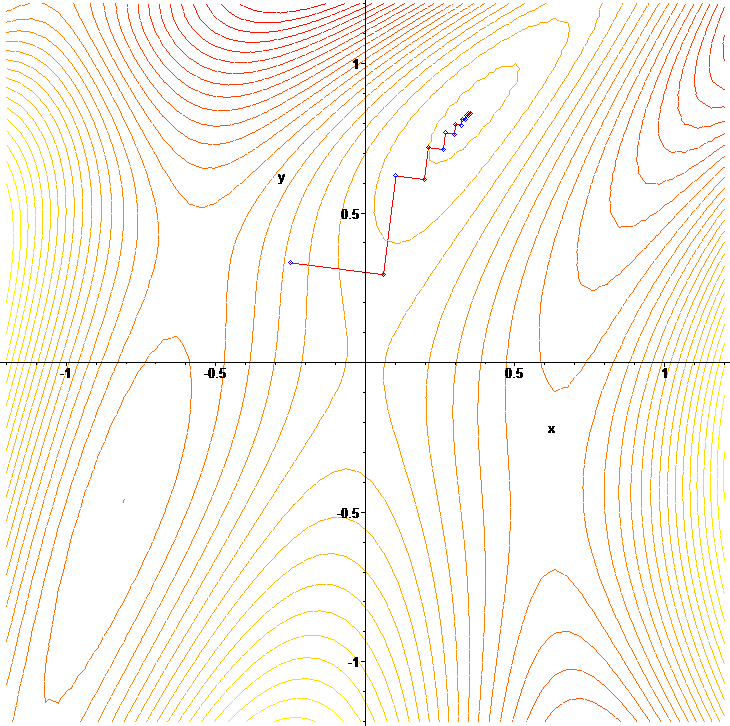
\includegraphics[width=0.45\textwidth]{images/gradient_ascent_contour.png}
  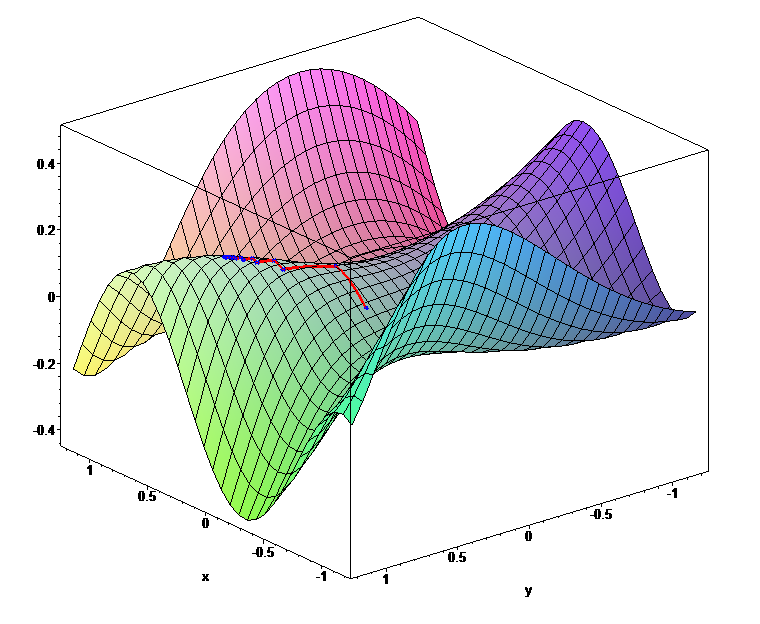
\includegraphics[width=0.45\textwidth]{images/gradient_ascent_surface.png}
  \caption{\label{fig:grad-desc}Visualización de la técnica de gradiente descendente, en este caso, buscando un máximo de la función $F(x,y)=\sin\left(\frac{1}{2} x^2 - \frac{1}{4} y^2 + 3 \right) \cos(2 x+1-e^y)$. Imágenes de Wikimedia Commons en dominio público}
\end{figure}

La técnica de gradiente descendente presenta algunos problemas: como se
puede observar en la \autoref{fig:grad-desc}, cuando el gradiente de
la función es próximo a cero el algoritmo tiende a dar pasos muy cortos,
convergiendo muy lentamente hacia el extremo local encontrado. Asimismo,
en general puede presentar un comportamiento de zigzag para ciertas
funciones, avanzando de forma casi ortogonal al segmento que guarda la
distancia más corta con el extremo.
